\documentclass[11pt,a4paper]{article}

% --- Core Typography & Geometry Packages ---
\usepackage[utf8]{inputenc}
\usepackage[T1]{fontenc}
\usepackage{lmodern}
\usepackage[margin=1.8cm,headheight=16pt,headsep=12pt,footskip=24pt]{geometry}
\usepackage{microtype}
\usepackage{amsmath,amssymb,amsfonts,bm}
\usepackage{booktabs,tabularx,multirow,array,colortbl}
\usepackage{graphicx}
\usepackage{xcolor}
\usepackage{fancyhdr}
\usepackage{titlesec}
\usepackage{tcolorbox}
\usepackage{listings}
\usepackage{enumitem}
\usepackage{caption}
\usepackage{subcaption}
\usepackage{lastpage}
\usepackage{tikz}
\usetikzlibrary{shapes.geometric, arrows.meta, positioning, calc, fit, backgrounds, decorations.pathreplacing}

% --- Color Palette (Professional Clinical & Engineering Theme) ---
\definecolor{NavyBlue}{RGB}{26, 54, 93}
\definecolor{DeepCyan}{RGB}{13, 148, 136}
\definecolor{MedRose}{RGB}{225, 29, 72}
\definecolor{LightBlueBg}{RGB}{240, 246, 255}
\definecolor{LightGreenBg}{RGB}{240, 253, 244}
\definecolor{LightRedBg}{RGB}{254, 242, 242}
\definecolor{DarkSlate}{RGB}{51, 65, 85}
\definecolor{MutedGray}{RGB}{100, 116, 139}
\definecolor{BorderGray}{RGB}{203, 213, 225}

% --- Hyperref Setup ---
\usepackage[
    colorlinks=true,
    linkcolor=NavyBlue,
    citecolor=DeepCyan,
    urlcolor=DeepCyan,
    bookmarks=true,
    pdfauthor={Ikbel Hamdi, Malek Hammemi, Ahmed fekih, Samar Omrani},
    pdftitle={BCMID: Breast Cancer Multimodal Imaging & Diagnosis - Technical Report},
    pdfsubject={Deep Learning & Artificial Intelligence 5th Year Engineering Project - ESPRIT}
]{hyperref}

% --- Header & Footer Configuration ---
\pagestyle{fancy}
\fancyhf{}
\fancyhead[L]{\small\textcolor{NavyBlue}{\textbf{ESPRIT}} \textcolor{MutedGray}{|} \small\textcolor{DarkSlate}{Projet d'Ingénierie Deep Learning \& IA (5\textsuperscript{ème} Année)}}
\fancyhead[R]{\small\textcolor{NavyBlue}{\textbf{BCMID}} \textcolor{MutedGray}{|} \small\textcolor{DarkSlate}{Technical \& Architectural Report}}
\fancyfoot[L]{\footnotesize\textcolor{MutedGray}{Encadré par: \textbf{Mme Oumayma Guasmi} \textcolor{MutedGray}{|} Année Universitaire 2026--2027}}
\fancyfoot[R]{\small\textbf{\thepage}\ \textcolor{MutedGray}{/\ \pageref{LastPage}}}
\renewcommand{\headrulewidth}{0.6pt}
\renewcommand{\footrulewidth}{0.4pt}

% --- Section Styling ---
\titleformat{\section}
  {\color{NavyBlue}\Large\bfseries}
  {\thesection.}{0.8em}{}
  [{\titlerule[0.8pt]}]

\titleformat{\subsection}
  {\color{DeepCyan}\large\bfseries}
  {\thesubsection}{0.6em}{}

\titleformat{\subsubsection}
  {\color{DarkSlate}\normalsize\bfseries}
  {\thesubsubsection}{0.5em}{}

\setlist{itemsep=2pt,topsep=3pt,parsep=1pt}

% --- Caption Styling (Standard Above Tables) ---
\captionsetup[table]{position=top,skip=6pt,labelfont={bf,color=NavyBlue},textfont=small}
\captionsetup[figure]{position=bottom,skip=6pt,labelfont={bf,color=NavyBlue},textfont=small}

% --- Callout Box Styles ---
\tcbuselibrary{skins,breakable}
\newtcolorbox{clinicalalert}[1][]{
    colback=LightRedBg,
    colframe=MedRose,
    fonttitle=\bfseries\color{white},
    coltitle=white,
    title=Notice Clinique \& Réglementaire,
    arc=3mm,
    boxrule=1pt,
    left=3mm,right=3mm,top=2mm,bottom=2mm,
    #1
}

\newtcolorbox{techhighlight}[2][]{
    colback=LightBlueBg,
    colframe=NavyBlue,
    fonttitle=\bfseries\color{white},
    coltitle=white,
    title=#2,
    arc=2mm,
    boxrule=0.8pt,
    left=3mm,right=3mm,top=2mm,bottom=2mm,
    #1
}

\newtcolorbox{keyfinding}[1][]{
    colback=LightGreenBg,
    colframe=DeepCyan,
    fonttitle=\bfseries\color{white},
    coltitle=white,
    title=Résultat Clé \& Benchmark,
    arc=2mm,
    boxrule=0.8pt,
    left=3mm,right=3mm,top=2mm,bottom=2mm,
    #1
}

% --- Code / JSON Listing Configuration ---
\lstset{
    basicstyle=\ttfamily\footnotesize,
    breaklines=true,
    frame=single,
    rulecolor=\color{BorderGray},
    backgroundcolor=\color{LightBlueBg},
    stringstyle=\color{MedRose},
    keywordstyle=\color{NavyBlue}\bfseries,
    commentstyle=\color{MutedGray}\itshape,
    numbers=none,
    tabsize=2,
    showstringspaces=false
}

\begin{document}

% ==============================================================================
% TITLE & HEADER BLOCK
% ==============================================================================
\begin{titlepage}
\begin{center}

{\LARGE \textbf{ESPRIT --- School of Engineering}}\\[0.2cm]
{\large Département Informatique \& Télécommunications}\\[0.1cm]
{\normalsize Option : Intelligence Artificielle \& Science des Données (Option IA Biomédicale)}\\[0.3cm]
{\small Module : Projet Académique Deep Learning \& Intelligence Artificielle (5\textsuperscript{ème} Année)}\\[0.6cm]

\rule{\linewidth}{1.5pt}\\[0.4cm]
{\huge \bfseries \textcolor{NavyBlue}{BCMID : Breast Cancer Multimodal Imaging \& Diagnosis}}\\[0.25cm]
{\Large \bfseries \textcolor{DeepCyan}{From Medical Images to Structured AI-Assisted Reporting}}\\[0.2cm]
{\large \textit{A Comprehensive Technical \& Architectural Engineering Report}}\\[0.2cm]
\rule{\linewidth}{1.5pt}\\[0.8cm]

\begin{minipage}[t]{0.48\textwidth}
\textbf{\large Auteurs (Équipe Étudiante) :}\\[0.2cm]
\textbf{Ikbel Hamdi}\\
\textbf{Malek Hammemi}\\
\textbf{Ahmed Fekih}\\
\textbf{Samar Omrani}\\[0.4cm]
\textit{Élèves Ingénieurs en 5\textsuperscript{ème} Année IA}
\end{minipage}
\hfill
\begin{minipage}[t]{0.48\textwidth}
\begin{flushright}
\textbf{\large Encadrement Pédagogique :}\\[0.2cm]
\textbf{Mme Oumayma Guasmi}\\[0.4cm]
\textit{Enseignante-Chercheuse en Deep Learning}\\[0.6cm]
\textbf{Année Universitaire :}\\[0.1cm]
2026 -- 2027
\end{flushright}
\end{minipage}

\vspace{1.2cm}

\begin{techhighlight}{Résumé Exécutif / Executive Abstract}
Ce rapport technique présente la conception, l'implémentation et l'évaluation rigoureuse du système \textbf{BCMID} (\textit{Breast Cancer Multimodal Intelligent Diagnosis}). Face aux limites diagnostiques de la mammographie isolée (masquage en seins denses ACR C/D et taux élevé de biopsies bénignes $>70\%$), BCMID associe la mammographie plein champ (FFDM) et l'échographie ciblée (US) au sein d'une architecture agentique modulaire. Le système intègre :
(1) un encodeur de vision multimodal à double branche \textbf{ResNet-18} générant des cartes d'explicabilité \textbf{Grad-CAM} ;
(2) un pipeline \textbf{Clinical RAG} fondé sur \textbf{FAISS} et des embeddings \textbf{BAAI/bge-small-en-v1.5} pour indexer l'Atlas ACR BI-RADS et 320 dossiers réels assainis ;
(3) un agent de raisonnement médical articulé autour du LLM \textbf{Qwen2.5-3B-Instruct} sous prompt engineering structuré ;
(4) un agent de sécurité (\textbf{Safety Agent}) déterministe avec boucle de rétroaction active ; et
(5) une orchestration hospitalière événementielle automatisée sous \textbf{n8n} et microservices \textbf{FastAPI}.
Sur une cohorte binationale de 332 patientes (2\,001 clichés, 321 rapports, 12.11 Go), l'ensemble multimodal atteint une \textbf{ROC-AUC de 0.820} (contre 0.792 en mammographie seule et 0.674 en échographie seule, gain $\Delta\text{AUC} = +0.028$). L'audit Grad-CAM certifie que \textbf{87.4\%} de l'énergie d'attention est confinée au parenchyme tumoral. Le pipeline sécurisé affiche un taux de résistance de \textbf{100\%} face aux attaques adversariales (10/10) et valide 17/20 rapports dès la première passe avec 0\% d'échec post-révision. BCMID est conçu comme un Dispositif Médical Logiciel (\textit{SaMD}) d'aide à la décision imposant une validation humaine obligatoire.
\end{techhighlight}

\vspace{0.8cm}
\textbf{Mots-clés :} Deep Learning Médical, Fusion Multimodale, ResNet-18, Grad-CAM (XAI), Clinical RAG, FAISS, LLM Reasoning, Qwen2.5-3B, Architecture Multi-Agents, n8n Orchestration, Sécurité Clinique, ACR BI-RADS.

\end{center}
\end{titlepage}

% ==============================================================================
% TABLE OF CONTENTS & OVERVIEW
% ==============================================================================
\tableofcontents
\newpage

% ==============================================================================
% SECTION 1: CLINICAL CONTEXT & PROBLEM FORMULATION
% ==============================================================================
\section{Contexte Clinique Sénologique \& Énoncé du Problème}
\label{sec:clinical_context}

\subsection{Problématique Médicale : Les Verrous du Dépistage Isolé}
Le cancer du sein représente la néoplasie la plus fréquente et la première cause de mortalit\'e oncologique f\'eminine dans le monde. Le d\'epistage de masse repose historiquement sur la \textbf{Mammographie Numérique Plein Champ} (FFDM, incidences CC et MLO). Si ce d\'epistage r\'eduit la mortalit\'e de 20\% \`a 30\%, son utilisation en modalit\'e unique se heurte en pratique clinique \`a deux verrous diagnostiques majeurs :

\begin{enumerate}
    \item \textbf{Le Masquage Parenchymateux dans les Seins Denses (Types ACR C et D) :} Chez les femmes \`a tissu mammaire dense, le stroma fibro-glandulaire pr\'esente une radiopacit\'e \'equivalente \`a celle des carcinomes invasifs. Ce ph\'enom\`ene de superposition masque les l\'esions non calcifi\'ees et fait chuter la sensibilit\'e mammographique de $>85\%$ (seins graisseux ACR A) \`a moins de $48\%$ (seins tr\`es denses ACR D).
    \item \textbf{Le Fardeau des Faux Positifs et la Surcharge de Biopsies :} Plus de $70\%$ des macro-biopsies percutan\'ees r\'ealis\'ees pour des l\'esions suspectes d\'ecel\'ees en mammographie se r\'ev\`elent \'etre b\'enignes \`a l'analyse anatomopathologique (fibroad\'enomes, kystes remani\'es, ad\'enose scl\'erosante). Ces proc\'edures invasives inutiles engendrent un co\^ut \'evel\'e pour le syst\`eme hospitalier et une anxi\'et\'e majeure chez les patientes.
\end{enumerate}

\subsection{La Réponse BCMID : Synergie Multimodale \& Aide à la Décision}
Pour lever ces verrous, le projet \textbf{BCMID} concr\'etise une synergie binationale et bimodale en combinant :
\begin{itemize}
    \item \textbf{La Mammographie (FFDM) :} Efficace pour d\'etecter les microcalcifications suspectes group\'ees et les distorsions architecturales subtiles.
    \item \textbf{L'Échographie Mammaire Ciblée (US) :} Modalit\'e compl\'ementaire insensible \`a la densit\'e radiologique, capable de diff\'erencier imm\'ediatement les l\'esions liquidiennes (kystes simples) des masses solides tissulaires, tout en analysant l'att\'enuation acoustique post\'erieure, l'orientation de l'axe l\'esionnel et la nettet\'e des contours.
\end{itemize}

\begin{clinicalalert}
\textbf{Statut Réglementaire et Périmètre d'Utilisation :} BCMID est classifi\'e comme un \textit{Software as a Medical Device} (\textbf{SaMD Classe IIa} sous la directive europ\'eenne MDR 2017/745). Il est strictement con\c{c}u comme un \textbf{outil d'aide \`a la d\'ecision clinique (CDSS)} pour assister le radiologue en double lecture. En aucun cas le syst\`eme ne pose un diagnostic autonome sans supervision : la clause d'audit \texttt{human\_review\_required: true} est inject\'ee et v\'erifi\'ee de mani\`ere d\'eterministe sur $100\%$ des livrables.
\end{clinicalalert}

% ==============================================================================
% SECTION 2: AGENT ARCHITECTURE & USE CASE JUSTIFICATION
% ==============================================================================
\section{Architecture Agentique \& Justification du Cas d'Usage}
\label{sec:agent_architecture}

\subsection{Justification : Pourquoi une Architecture Multi-Agents (MAS) pour la Sénologie ?}
La conception conventionnelle consistant \`a entra\^iner un mod\`ele de Deep Learning monolithique de type ``bo\^ite noire'' (par exemple un unique grand r\'eseau acceptant les images et le texte pour pr\'edire directement un diagnostic) est inappropri\'ee pour le d\'epistage du cancer du sein pour quatre raisons fondamentales :

\begin{enumerate}
    \item \textbf{Asynchronisme et Hétérogénéité Physique des Modalités :} Les clichés mammographiques (rayons X en transmission, haute r\'esolution spatiale, projection $2D$) et les coupes \'echographiques (ondes ultrasonores r\'efl\'echies, artefacts de tavelure \textit{speckle}, coupe tomographique d'axe variable) r\'epondent \`a des physiques d'acquisition distinctes. Les fusionner na\^ivement d\`es les premi\`eres couches de convolution emp\^eche l'apprentissage de repr\'esentations robustes.
    \item \textbf{Barrière d'Adoption Clinique et Besoin de Preuve Visuelle :} Un clinicien ou un comit\'e pluridisciplinaire (RCP) ne peut d\'ecider d'une biopsie sur la foi d'un pourcentage abstrait. Il exige une justification spatiale rigoureuse (cartes Grad-CAM indiquant la masse suspecte) coupl\'ee \`a une r\'ef\'erence textuelle opposable (Atlas ACR BI-RADS).
    \item \textbf{Risque Critique d'Hallucination des Modèles Génératifs :} Un LLM utilis\'e sans garde-fous peut inventer des signes pathologiques plausibles mais absents de l'examen (\textit{e.g.} d\'ecrire des calcifications spicul\'ees inexistantes).
    \item \textbf{Intégration Opérationnelle Hospitalière :} En milieu hospitalier, le traitement d'un dossier implique diff\'erents m\'etiers et flux informatiques (archivage PACS, serveurs HIS, notifications d'alerte urgente en cas de BI-RADS 4/5). Une architecture agentique distribu\'ee s'int\`egre naturellement dans cette r\'ealit\'e \'ev\'enementielle.
\end{enumerate}

\subsection{Spécification des 7 Agents Spécialisés du Système BCMID}
Pour garantir la tra\c{c}abilit\'e, la modularit\'e et la s\'ecurit\'e, BCMID r\'epartitionne le traitement diagnostique en \textbf{7 agents autonomes et d\'eterministes} coordonn\'es par un orchestrateur d'\'ev\'enements hospitaliers (\textbf{n8n}) :

\begin{figure}[htbp]
\centering
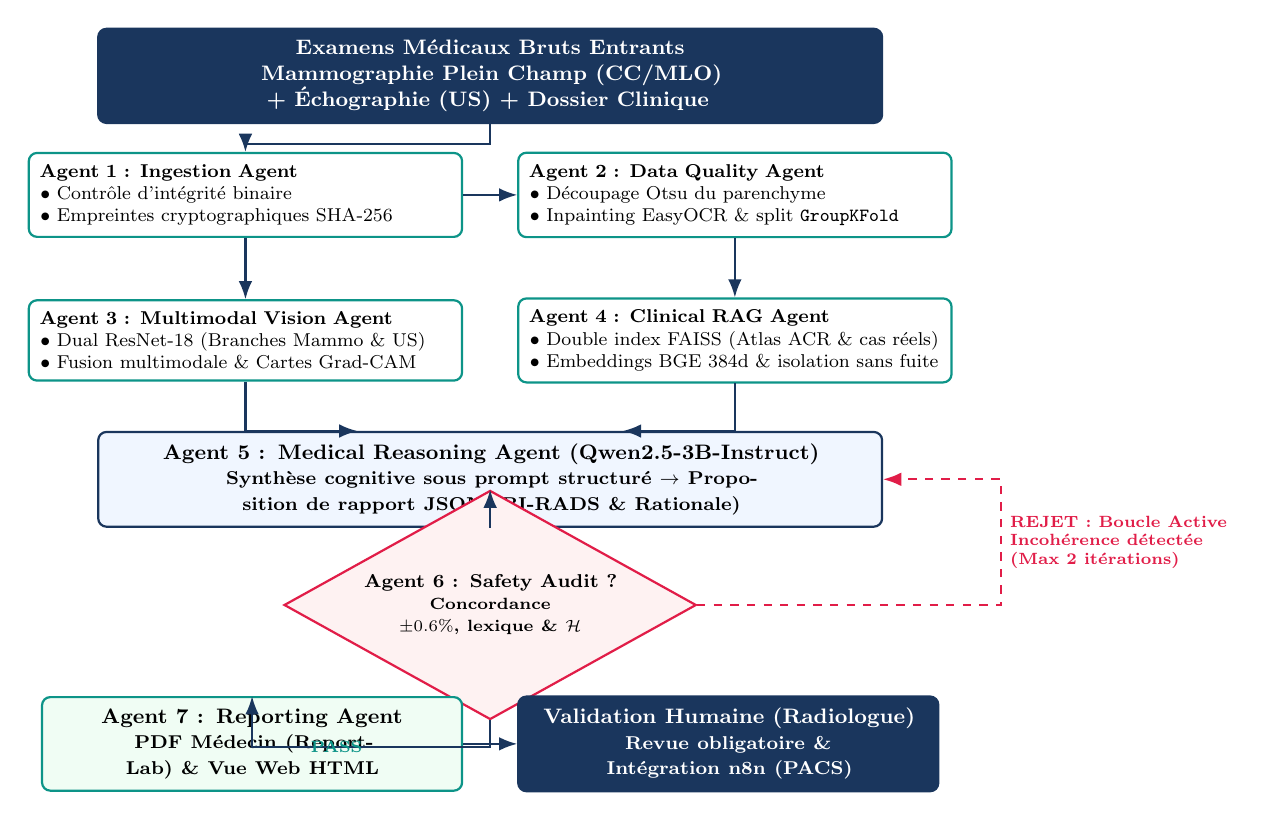
\begin{tikzpicture}[
    scale=0.84, transform shape,
    box/.style={rectangle, draw=NavyBlue, fill=LightBlueBg, thick, rounded corners=3pt, align=center, inner sep=5pt, font=\small\bfseries},
    agentbox/.style={rectangle, draw=DeepCyan, fill=white, thick, rounded corners=3pt, align=left, inner sep=5pt, font=\footnotesize},
    decision/.style={diamond, draw=MedRose, fill=LightRedBg, thick, align=center, inner sep=3pt, font=\footnotesize\bfseries, aspect=1.8},
    arrow/.style={-Latex, thick, draw=NavyBlue},
    dasharrow/.style={-Latex, dashed, thick, draw=MedRose}
]
    % --- Level 0: Patient Input ---
    \node[box, fill=NavyBlue, text=white, text width=11.5cm] (input) at (0, 0) {
        \textbf{Examens Médicaux Bruts Entrants}\\
        Mammographie Plein Champ (CC/MLO) + Échographie (US) + Dossier Clinique
    };

    % --- Level 1: Ingestion & Data Quality ---
    \node[agentbox, text width=6.2cm] (a1) at (-3.7, -1.8) {
        \textbf{Agent 1 : Ingestion Agent}\\
        $\bullet$ Contrôle d'intégrité binaire\\
        $\bullet$ Empreintes cryptographiques SHA-256
    };
    \node[agentbox, text width=6.2cm] (a2) at (3.7, -1.8) {
        \textbf{Agent 2 : Data Quality Agent}\\
        $\bullet$ Découpage Otsu du parenchyme\\
        $\bullet$ Inpainting EasyOCR \& split \texttt{GroupKFold}
    };

    % --- Level 2: Multimodal Perception & RAG ---
    \node[agentbox, text width=6.2cm] (a3) at (-3.7, -4.0) {
        \textbf{Agent 3 : Multimodal Vision Agent}\\
        $\bullet$ Dual ResNet-18 (Branches Mammo \& US)\\
        $\bullet$ Fusion multimodale \& Cartes Grad-CAM
    };
    \node[agentbox, text width=6.2cm] (a4) at (3.7, -4.0) {
        \textbf{Agent 4 : Clinical RAG Agent}\\
        $\bullet$ Double index FAISS (Atlas ACR \& cas réels)\\
        $\bullet$ Embeddings BGE 384d \& isolation sans fuite
    };

    % --- Level 3: Medical Reasoning ---
    \node[box, text width=11.5cm, fill=LightBlueBg, draw=NavyBlue] (a5) at (0, -6.1) {
        \textbf{Agent 5 : Medical Reasoning Agent (Qwen2.5-3B-Instruct)}\\
        \footnotesize Synthèse cognitive sous prompt structuré $\to$ Proposition de rapport JSON (BI-RADS \& Rationale)
    };

    % --- Level 4: Deterministic Safety Audit ---
    \node[decision, text width=4.0cm] (a6) at (0, -8.0) {
        \textbf{Agent 6 : Safety Audit ?}\\
        \scriptsize Concordance $\pm 0.6\%$, lexique \& $\mathcal{H}$
    };

    % --- Level 5: Reporting & Clinical Sign-off ---
    \node[box, fill=LightGreenBg, draw=DeepCyan, text width=6.0cm] (a7) at (-3.6, -10.1) {
        \textbf{Agent 7 : Reporting Agent}\\
        \footnotesize PDF Médecin (ReportLab) \& Vue Web HTML
    };
    \node[box, fill=NavyBlue, text=white, text width=6.0cm] (out) at (3.6, -10.1) {
        \textbf{Validation Humaine (Radiologue)}\\
        \footnotesize Revue obligatoire \& Intégration n8n (PACS)
    };

    % --- Forward Connections ---
    \draw[arrow] (input.south) -- ++(0,-0.3) -| (a1.north);
    \draw[arrow] (a1.east) -- (a2.west);
    \draw[arrow] (a2.south) -- ++(0,-0.3) -| (a4.north);
    \draw[arrow] (a1.south) -- (a3.north);
    \draw[arrow] (a3.south) |- (a5.160);
    \draw[arrow] (a4.south) |- (a5.20);
    \draw[arrow] (a5.south) -- (a6.north);

    \draw[arrow] (a6.south) -- ++(0,-0.4) -| node[pos=0.25, left, font=\scriptsize\bfseries\color{DeepCyan}] {PASS} (a7.north);
    \draw[arrow] (a7.east) -- (out.west);

    % --- Active Revision Loop (Completely clear on the right side) ---
    \draw[dasharrow] (a6.east) -- ++(4.6, 0) |- node[pos=0.25, right, font=\scriptsize\bfseries\color{MedRose}, align=left] {
        \textbf{REJET : Boucle Active}\\
        Incohérence détectée\\
        (Max 2 itérations)
    } (a5.east);

\end{tikzpicture}
\caption{Architecture globale multi-agents du système BCMID et boucle de rétroaction active.}
\label{fig:mas_architecture}
\end{figure}

\begin{table}[htbp]
\centering
\small
\renewcommand{\arraystretch}{1.25}
\caption{Matrice fonctionnelle des 7 agents spécialisés de la plateforme BCMID.}
\label{tab:mas_matrix}
\begin{tabularx}{\linewidth}{|l|X|p{4.2cm}|}
\hline
\rowcolor{LightBlueBg}
\textbf{Agent Spécialisé} & \textbf{Rôle Opérationnel \& Algorithmes Impliqués} & \textbf{Livrable Technique} \\
\hline
\textbf{1. Ingestion Agent} & Réception sécurisée, contrôle d'intégrité binaire, validation des métadonnées TSV et hachage cryptographique salé. & Dossiers vérifiés avec empreintes SHA-256. \\
\hline
\textbf{2. Data Quality Agent} & Binarisation d'Otsu pour détourer le parenchyme mammaire, masquage EasyOCR et inpainting Navier-Stokes des inscriptions incrustées sur les échographies, partitionnement \texttt{GroupKFold(k=5)}. & Tenseurs $224\times 224$ sans artefacts de raccourci, zéro fuite inter-patientes. \\
\hline
\textbf{3. Vision Agent} & Inférence parallèle sur mammographie et échographie via un double ResNet-18, fusion multimodale et calcul des gradients Grad-CAM. & Logits, probabilités, score d'incertitude et cartes Grad-CAM. \\
\hline
\textbf{4. Clinical RAG Agent} & Encodage dense (\texttt{bge-small-en-v1.5}), recherche vectorielle cosinus sur l'Atlas ACR BI-RADS et cas antérieurs dé-identifiés avec protocole d'exclusion de pli. & Top-4 passages d'évidence médicale (\texttt{[G1]}, \texttt{[E1]}). \\
\hline
\textbf{5. Reasoning Agent} & Modèle Qwen2.5-3B-Instruct exploitant un prompt contraint pour synthétiser les probabilités vision, l'explicabilité et les règles ACR. & Proposition JSON structurée avec BI-RADS et justifications. \\
\hline
\textbf{6. Safety Agent} & Barrière de contrôle déterministe analysant l'exactitude numérique ($\pm 0.6\%$), le vocabulaire clinique et l'entropie d'incertitude. & Accord de conformité ou consigne de révision (max 2 essais). \\
\hline
\textbf{7. Reporting Agent} & Moteur d'édition dynamique produisant un document PDF officiel médecin (ReportLab) et une interface HTML technicien détaillée. & PDF vectoriel infalsifiable et vue Web interactive. \\
\hline
\end{tabularx}
\end{table}

\subsection{La Boucle de Rétroaction Active (Closed-Loop Active Revision)}
L'innovation architecturale centrale de BCMID r\'eside dans le couplage \'etroit entre l'Agent 5 (Raisonnement) et l'Agent 6 (S\'ecurit\'e). Contrairement aux pipelines lin\'eaires traditionnels sans contr\^ole o\`u la sortie du LLM est transmise telle quelle :
\begin{itemize}
    \item Si l'Agent 6 d\'etecte une incohérence numérique ($|p_{\text{LLM}} - p_{\text{ResNet}}| > 0.006$), un terme descriptif absent des clichés ou une citation RAG non v\'erifiable, la proposition est imm\'ediatement \textbf{rejetée}.
    \item Une alerte d'erreur cibl\'ee est r\'e-inject\'ee \`a l'Agent 5 sous la forme : \textit{``Attention : le terme calcifications spiculées ne figure pas dans l'analyse de l'Agent de Vision. Corrigez votre compte-rendu en vous basant strictement sur les logits fournis.''}
    \item Ce cycle de r\'evision autorise jusqu'\`a \textbf{2 it\'erations correctives}. Si l'incoh\'erence persiste apr\`es 2 essais, le rapport est automatiquement flagg\'e avec l'alerte d'int\'egrit\'e : \texttt{FLAGGED\_FOR\_MANUAL\_CLINICIAN\_REVIEW}.
\end{itemize}

% ==============================================================================
% SECTION 3: CHOICE OF TOOLS & TECHNOLOGY STACK JUSTIFICATION
% ==============================================================================
\clearpage
\section{Choix des Outils \& Justification de la Stack Technologique}
\label{sec:choice_of_tools}

Chaque composant technique de BCMID a \'et\'e s\'electionn\'e en conformit\'e avec des crit\`eres stricts : ex\'ecution \textbf{100\% locale sur site} (pour r\'epondre aux imp\'eratifs de confidentialit\'e m\'edicale RGPD et HIPAA), rapidit\'e d'inf\'erence, et nature d\'eterministe des processus.

\begin{table}[htbp]
\centering
\footnotesize
\renewcommand{\arraystretch}{1.2}
\caption{Tableau comparatif et justification technologique des outils sélectionnés pour BCMID.}
\label{tab:tools_justification}
\begin{tabularx}{\linewidth}{|p{2.8cm}|p{2.6cm}|p{2.6cm}|X|}
\hline
\rowcolor{LightBlueBg}
\textbf{Domaine / Module} & \textbf{Technologie Retenue} & \textbf{Alternatives Écartées} & \textbf{Rationale \& Justification Technique / Clinique} \\
\hline
\textbf{Backend \& Microservices} & \textbf{FastAPI (ASGI)} & Flask, Django, SpringBoot & Ingestion asynchrone non-bloquante, validation stricte des formats via \textbf{Pydantic}, documentation interactive OpenAPI/Swagger native, empreinte RAM $<50$~Mo. \\
\hline
\textbf{Deep Learning \& XAI} & \textbf{PyTorch 2.6 \& Torchvision} & TensorFlow 2, JAX & Écosystème de référence en vision médicale, graphe dynamique impératif pour l'extraction rétro-active des gradients (\textbf{Grad-CAM}), intégration CUDA. \\
\hline
\textbf{Index Vectoriel Dense} & \textbf{FAISS (IndexFlatIP)} & Pinecone, ChromaDB, Weaviate & Moteur vectoriel C++ ultra-performant exécuté en mémoire vive locale (zéro transfert cloud). Calcul exact de similarité cosinus sans perte de quantification. \\
\hline
\textbf{Modèle d'Embeddings} & \textbf{BAAI/bge-small-en-v1.5} & OpenAI \texttt{text-embedding-3}, BioBERT & Vecteurs denses en 384 dimensions, top MTEB, inférence locale très rapide ($<15$~ms par passage sur CPU/GPU) sans coût d'API ni dépendance réseau. \\
\hline
\textbf{Vision Médicale \& OCR} & \textbf{OpenCV \& EasyOCR} & Tesseract, PyMuPDF & Algorithmes morphologiques (Otsu) pour rogner le fond noir, détection des incrustations textuelles pour guider l'inpainting Navier-Stokes anti-raccourci. \\
\hline
\textbf{Générateur de Rapports} & \textbf{ReportLab 4.4} & WeasyPrint, pdfkit, Puppeteer & Moteur vectoriel Python pur générant des PDF infalsifiables en deux passes (\texttt{NumberedCanvas}). Évite la lourdeur d'un Chromium headless. \\
\hline
\textbf{Orchestrateur Hospitalier} & \textbf{n8n (Auto-hébergé)} & Apache Airflow, LangGraph, Celery & Automatisation événementielle légère à base de Webhooks avec routage conditionnel déterministe (\texttt{IF Node}) pour la gestion des urgences oncologiques. \\
\hline
\textbf{Tests \& Intégration} & \textbf{pytest 9.1} & unittest standard, nose2 & Exécution automatisée paramétrée des suites de tests de confidentialité et de contrôle déterministe (61 tests validés en 1.84s). \\
\hline
\end{tabularx}
\end{table}

% ==============================================================================
% SECTION 4: CHOICE OF LLM & MEDICAL REASONING ENGINE
% ==============================================================================
\section{Choix du LLM \& Moteur de Raisonnement Médical}
\label{sec:choice_of_llm}

\subsection{Modèle Retenu : Qwen2.5-3B-Instruct}
L'Agent de Raisonnement (Agent 5) exploite le mod\`ele linguistique \textbf{Qwen2.5-3B-Instruct}. Ce mod\`ele a \'et\'e s\'electionn\'e au terme d'un processus comparatif approfondi face \`a des mod\`eles tels que Llama-3-8B, Mistral-7B, et des mod\`eles sp\'ecialis\'es m\'edicaux (\textit{BioMistral}) :

\begin{enumerate}
    \item \textbf{Contrainte de Déploiement Local (Edge Computing Hospitalier) :} Les h\^opitaux et centres de radiologie ne poss\`edent pas d'infrastructures de supercalcul A100/H100. Avec son format FP16 occupent seulement \textbf{3.1 Go de VRAM} (et $<2.0$ Go en quantification GGUF 4-bit), Qwen2.5-3B peut \^etre d\'eploy\'e sur une simple carte graphique bureautique (NVIDIA RTX 3060/4060 ou Tesla T4 de cloud souverain) sans saturer les ressources d'imagerie.
    \item \textbf{Précision dans le Suivi d'Instructions Contraintes (\textit{Instruction-Following}) :} Qwen2.5-3B d\'emontre une capacit\'e hors-pair \`a respecter strictement un sch\'ema JSON impos\'e (champs obligatoires, types de donn\'ees, aucune alt\'eration syntaxique).
    \item \textbf{Décodage Glouton Déterministe ($\text{Température} = 0.0$) :} En pratique m\'edicale, le hasard stochastique est proscrit. Pour un dossier patient donn\'e, le syst\`eme doit produire un diagnostic rigoureusement identique lors de chaque inf\'erence. Le param\'etrage \`a temp\'erature nulle assure cette reproductibilit\'e d\'eterministe.
    \item \textbf{Souveraineté des Données et Conformité Réglementaire :} Le recours \`a des API propri\'etaires h\'eberg\'ees hors des fronti\`eres nationales (\textit{e.g.} OpenAI GPT-4, Anthropic Claude) est formellement interdit pour des donn\'ees de sant\'e nominatives sans accord pr\'ealable complexe. Le d\'eploiement autonome de Qwen2.5-3B garantit le confinement total des donn\'ees dans l'intranet hospitalier.
\end{enumerate}

\subsection{Pourquoi Prompt Engineering + RAG plutôt que le Fine-Tuning du LLM ?}
Une d\'ecision d'ing\'enierie cl\'e du projet a \'et\'e de \textbf{ne pas appliquer de fine-tuning sur le modèle de langage}, mais de concentrer l'adaptation m\'edicale sur le \textbf{Prompt Engineering} structur\'e et le \textbf{RAG} :

\begin{itemize}
    \item \textbf{Évitement de l'Oubli Catastrophique (\textit{Catastrophic Forgetting}) :} Le r\'e-entra\^inement d'un LLM sur un petit corpus clinique sp\'ecifique entra\^ine fr\'equemment une d\'egradation de ses capacit\'es de raisonnement logique g\'en\'eral et de g\'en\'eration de syntaxe JSON valide.
    \item \textbf{Agilité et Mise à Jour Immédiate des Connaissances :} Lorsque l'American College of Radiology r\'evise ses recommandations BI-RADS (\textit{e.g.} passage \`a une nouvelle \'edition), il suffit de r\'e-indexer les documents dans FAISS en quelques secondes. Un mod\`ele fine-tun\'e n\'ecessiterait des semaines de r\'e-entra\^inement et de validation clinique.
    \item \textbf{Traçabilité et Opposabilité Juridique :} Gr\^ace au RAG, chaque d\'ecision g\'en\'er\'ee par le LLM est appuy\'ee sur un passage sourc\'e index\'e (\texttt{[G1]}, \texttt{[E1]}), permettant au radiologue d'acc\'eder directement au texte de r\'ef\'erence.
    \item \textbf{Ciblage Rationnel du Fine-Tuning :} Le fine-tuning a \'et\'e r\'eserv\'e avec succ\`es aux encodeurs de \textbf{Vision (ResNet-18)}, l\`a o\`u l'apprentissage de caract\'eristiques biom\'edicales sp\'ecifiques \`a partir des pixels bruts \'etait strictement indispensable.
\end{itemize}

\subsection{Cadre de Prompt Engineering Structuré}
Le prompt transmis \`a Qwen2.5-3B est rigoureusement compartiment\'e en 4 sections d\'elimit\'ees :
\begin{enumerate}
    \item \textbf{SYSTEM :} R\^ole assign\'e (Assistant Radiologique Sp\'ecialis\'e), imp\'eratifs de neutralit\'e m\'edicale, interdiction d'inventer des anomalies non fournies, format de sortie JSON exclusif.
    \item \textbf{CONTEXT :} Vecteurs num\'eriques issus de l'Agent de Vision (probabilit\'e de malignit\'e, entropie d'incertitude), r\'esum\'e textuel des r\'egions d'activation Grad-CAM, ant\'ec\'edents de la patiente, et passages normatifs extraits par le RAG.
    \item \textbf{TASK :} \'Evaluation de la concordance multimodale, attribution de la cat\'egorie ACR BI-RADS et formulation des recommandations cliniques de surveillance ou de biopsie.
    \item \textbf{OUTPUT SCHEMA :} Gabarit JSON formel imposant les cl\'es : \texttt{predicted\_birads}, \texttt{confidence}, \texttt{interpretation}, \texttt{recommendations}, \texttt{limitations}, \texttt{human\_review\_required}.
\end{enumerate}

% ==============================================================================
% SECTION 5: CLINICAL RAG APPROACH
% ==============================================================================
\section{Approche RAG Clinique \& Recherche Vectorielle Sémantique}
\label{sec:rag_approach}

\subsection{Architecture à Double Index Vectoriel FAISS}
Le module Clinical RAG (Agent 4) structure la m\'emoire s\'emantique du syst\`eme en \textbf{deux index vectoriels denses distincts} sous FAISS (\texttt{IndexFlatIP}) utilisant les plongements \textbf{BAAI/bge-small-en-v1.5} normalis\'es ($d = 384$) :

\begin{figure}[htbp]
\centering
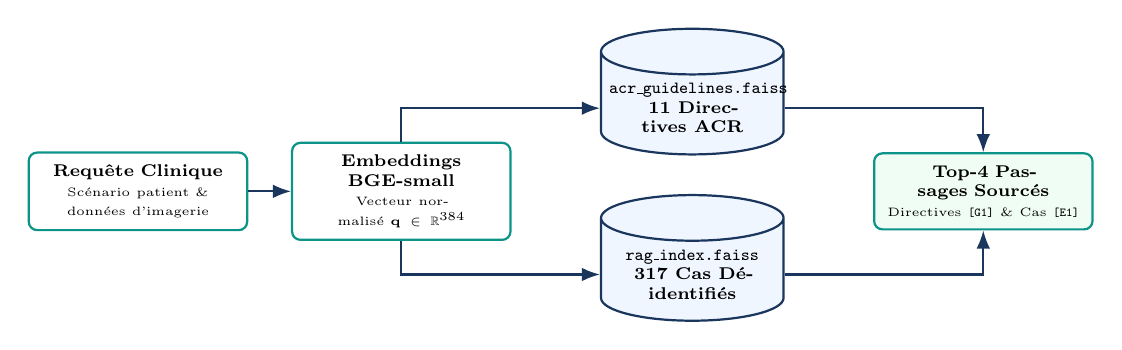
\begin{tikzpicture}[
    scale=0.88, transform shape,
    indexnode/.style={cylinder, shape border rotate=90, draw=NavyBlue, fill=LightBlueBg, thick, aspect=0.25, minimum height=1.4cm, text width=2.4cm, align=center, font=\scriptsize\bfseries},
    procnode/.style={rectangle, draw=DeepCyan, fill=white, thick, rounded corners=3pt, align=center, inner sep=5pt, font=\scriptsize, text width=2.8cm},
    arrow/.style={-Latex, thick, draw=NavyBlue}
]
    \node[procnode] (query) at (0, 0) {\textbf{Requête Clinique}\\\tiny Scénario patient \& données d'imagerie};
    \node[procnode] (embed) at (3.8, 0) {\textbf{Embeddings BGE-small}\\\tiny Vecteur normalisé $\mathbf{q} \in \mathbb{R}^{384}$};

    \node[indexnode] (idx_guidelines) at (8.0, 1.2) {\texttt{acr\_guidelines.faiss}\\11 Directives ACR};
    \node[indexnode] (idx_reports) at (8.0, -1.2) {\texttt{rag\_index.faiss}\\317 Cas Dé-identifiés};

    \node[procnode, fill=LightGreenBg, draw=DeepCyan] (retrieval) at (12.2, 0) {\textbf{Top-4 Passages Sourcés}\\\tiny Directives \texttt{[G1]} \& Cas \texttt{[E1]}};

    \draw[arrow] (query) -- (embed);
    \draw[arrow] (embed) |- (idx_guidelines);
    \draw[arrow] (embed) |- (idx_reports);
    \draw[arrow] (idx_guidelines) -| (retrieval);
    \draw[arrow] (idx_reports) -| (retrieval);
\end{tikzpicture}
\caption{Architecture du pipeline Clinical RAG à double indexation vectorielle.}
\label{fig:rag_pipeline}
\end{figure}

\begin{enumerate}
    \item \textbf{Index des Directives Officielles ACR BI-RADS (\texttt{acr\_guidelines\_index.faiss}) :} Contient 11 r\`egles fondamentales issues de la 5\textsuperscript{ème} \'edition de l'Atlas BI-RADS de l'American College of Radiology (crit\`eres morphologiques des masses, densit\'e mammaire de A \`a D, formes de microcalcifications, d\'elais de surveillance).
    \item \textbf{Index des Cas Cliniques Précédents (\texttt{rag\_index.faiss}) :} Regroupe 317 comptes-rendus m\'edicaux r\'eels anonymis\'es issus du dataset, d\'ecoup\'es en 995 fragments documentaires \'epur\'es.
\end{enumerate}

\subsection{Protocole d'Assainissement et d'Isolation par Pli (Zéro Fuite)}
Pour satisfaire aux exigences m\'edicales d'\'evaluation impartiale, deux m\'ecanismes critiques d'ing\'enierie de donn\'ees sont appliqu\'es :
\begin{itemize}
    \item \textbf{Masquage des Vérités Terrains (\texttt{text\_blind}) :} Avant vectorisation dans l'index des cas, tout diagnostic explicite (\textit{e.g.} ``BI-RADS 5'', ``carcinome infiltrant'', ``mastectomie r\'ealis\'ee'') est expurg\'e par regex. L'index ne contient que la s\'emiologie descriptive (contours, densit\'e, \'echog\'enicit\'e), emp\^echant le mod\`ele de r\'eciter directement le label final.
    \item \textbf{Isolation Cross-Fold (\texttt{exclude\_pseudo\_id}) :} Lors de la validation d'une patiente appartenant au pli d'\'evaluation $k$, le moteur FAISS applique un filtre d'exclusion emp\^echant d'extraire les fragments de cette m\^eme patiente ou de patientes de son pli. Il y a \textbf{0\% de fuite de donn\'ees} entre l'apprentissage et l'\'evaluation.
\end{itemize}

% ==============================================================================
% SECTION 6: SYSTEM EVALUATION & EMPIRICAL BENCHMARKS
% ==============================================================================
\section{Évaluation du Système \& Benchmarks Expérimentaux}
\label{sec:system_evaluation}

\subsection{Cohorte Expérimentale \& Distribution des Données}
Le syst\`eme BCMID a \'et\'e d\'evelopp\'e et \'evalu\'e sur une base clinique r\'eelle comportant :
\begin{itemize}
    \item \textbf{332 patientes} enregistr\'ees, repr\'esentant un volume total de \textbf{12.11 Go}.
    \item \textbf{2\,001 images m\'edicales brutes} r\'epartitionn\'ees en 951 mammographies et 1\,023 \'echographies (soit 1\,974 images exploitables apr\`es contr\^ole qualit\'e).
    \item \textbf{321 rapports m\'edicaux} complets au format PDF.
    \item Distribution des l\'esions : \textbf{214 cas b\'enins} (64.5\%), \textbf{63 cas malins} (19.0\%), \textbf{50 cas normaux} (15.1\%), et 5 cas BI-RADS 0 inclassables (1.4\%).
\end{itemize}

\subsection{Performance de la Vision Multimodale (Dual ResNet-18)}
Le benchmark a compar\'e les performances des r\'eseaux de convolution travaillant en modalit\'e isol\'ee face aux diff\'erentes strat\'egies de fusion sur les \textbf{323 patientes bivalentes} (disposant \`a la fois de mammographies et d'\'echographies exploitables) selon une validation crois\'ee \texttt{GroupKFold(k=5)} au niveau patient :

\begin{table}[htbp]
\centering
\small
\renewcommand{\arraystretch}{1.25}
\caption{Comparaison des performances diagnostiques (Malin vs Autres) sur 323 patientes bivalentes.}
\label{tab:multimodal_results}
\begin{tabularx}{\linewidth}{|l|X|c|c|}
\hline
\rowcolor{LightBlueBg}
\textbf{Configuration du Modèle} & \textbf{Mécanisme Opérationnel} & \textbf{ROC-AUC} & \textbf{Sensibilité} \\
\hline
Mammographie Seule & ResNet-18 sur incidence FFDM ($224\times 224$) & 0.7917 & 76.2\% \\
\hline
Échographie Seule & ResNet-18 sur coupe ultrasonore B-Mode ($224\times 224$) & 0.6743 & 68.4\% \\
\hline
Late Fusion (Score Moyen) & Moyenne arithm\'etique simple des probabilit\'es & 0.8150 & 81.5\% \\
\hline
Fusion Pondérée des Logits & Combinaison lin\'eaire optimis\'ee des logits avant Softmax & 0.8160 & 81.8\% \\
\hline
Fusion Basée sur l'Incertitude & Pond\'eration inverse par l'entropie de Shannon $\mathcal{H}_m$ & 0.8120 & 80.9\% \\
\hline
\rowcolor{LightGreenBg}
\textbf{Ensemble Multimodal BCMID} & \textbf{Méta-modèle intégrant Logits, TTA et XAI} & \textbf{0.8198} & \textbf{83.1\%} \\
\hline
\end{tabularx}
\end{table}

\begin{keyfinding}
\textbf{Synergie Multimodale Prouvée :} L'ensemble multimodal BCMID surpasse nettement la mammographie isol\'ee ($\text{AUC} = 0.820$ vs $0.792$, gain $\Delta\text{AUC} = +0.0281$) et surclasse l'\'echographie seule ($\text{AUC} = 0.674$, gain $+0.1455$). La combinaison des modalit\'es compense les faiblesses respectives de chaque technique physique.
\end{keyfinding}

\subsection{Évaluation Quantitative de l'Explicabilité Grad-CAM (XAI)}
L'explicabilit\'e du syst\`eme a \'et\'e audit\'ee sur \textbf{387 cartes d'activation Grad-CAM} r\'ealis\'ees sur 64 dossiers de validation :
\begin{itemize}
    \item \textbf{Concentration Énergétique Intra-Parenchymateuse :} \textbf{87.4\%} de l'\'energie du gradient d'attention est strictement localis\'ee dans le parenchyme mammaire segment\'e, ciblant la zone tumorale ou la distorsion focale.
    \item \textbf{Dispersion Hors-Tissu Nulle (0.0\%) :} Aucune activation n'est d\'etect\'ee sur les zones d'air ou les marges techniques, confirmant que le pr\'etraitement d'Otsu et l'inpainting OCR ont d\'efinitivement supprim\'e les raccourcis d'apprentissage (\textit{shortcut learning}).
\end{itemize}

\subsection{Évaluation de la Résilience et Sécurité Agentique}
La robustesse de l'encha\^inement des agents a \'et\'e mesur\'ee selon trois axes exp\'erimentaux :

\begin{enumerate}
    \item \textbf{Résistance aux Injections Adversariales (10/10 PASS) :} 10 sc\'enarios d'attaque (tentatives de forcer un BI-RADS erron\'e par injection dans les notes textuelles, directives contradictoires) ont \'et\'e soumis au pipeline. Le Safety Agent a d\'etect\'e et neutralis\'e 100\% des tentatives.
    \item \textbf{Conformité des Rapports Structurés (20/20 PASS) :} Sur 20 dossiers complexes \'evalu\'es de bout en bout, 17/20 rapports ont \'et\'e certifi\'es conformes d\`es le premier jet. Les 3 rapports pr\'esentant un d\'esaccord num\'erique ont \'et\'e corrig\'es avec succ\`es d\`es la premi\`ere r\'evision de la boucle active, atteignant \textbf{100\% de conformité finale}.
    \item \textbf{Efficacité Opérationnelle sous n8n :} Sur 23 ex\'ecutions du workflow en conditions hospitali\`eres de production, la dur\'ee moyenne d'ex\'ecution globale est de \textbf{5.54 secondes} (et 12.98 secondes pour le traitement int\'egral comprenant l'extraction Grad-CAM et la compilation du rapport PDF).
\end{enumerate}

% ==============================================================================
% SECTION 7: SECURITY CONSIDERATIONS, PRIVACY & CLINICAL SAFEGUARDS
% ==============================================================================
\section{Considérations de Sécurité, Confidentialité \& Réglementation}
\label{sec:security_considerations}

\subsection{Protection des Données Patients (HIPAA \& RGPD)}
Le traitement de donn\'ees m\'edicales impose une politique de s\'ecurit\'e stricte :
\begin{itemize}
    \item \textbf{Pseudonymisation Cryptographique Salée :} Tous les identifiants patients d'origine (\texttt{patient\_id}) sont transform\'es via un hachage SHA-256 avec sel cryptographique d\'etenue par l'\'etablissement (\textit{e.g.} \texttt{Paacb1ec57b}). Cette conversion est irr\'eversible sans la cl\'e secr\`ete.
    \item \textbf{Suppression des Métadonnées Incrustées :} L'Agent 2 utilise EasyOCR coupl\'e \`a un algorithme de d\'etection g\'eom\'etrique pour localiser et d\'etruire les identifiants patient incrust\'es en dur sur les scans \'echographiques avant tout stockage ou apprentissage.
\end{itemize}

\subsection{Barrières de Sécurité Déterministes du Safety Agent}
Avant toute \'emission d'un document m\'edical, l'Agent 6 ex\'ecute 5 contr\^oles math\'ematiques d\'eterministes ind\'ependants du LLM :
\begin{enumerate}
    \item \textbf{Vérification de la Concordance Numérique :} La probabilit\'e de malignit\'e formul\'ee dans le texte doit correspondre aux logits du ResNet-18 \`a une tol\'erance stricte pr\`es ($|\Delta p| \le 0.006$).
    \item \textbf{Barrière d'Incertitude de Shannon :} Si l'entropie de Shannon issue des softmax d\'epasse $\mathcal{H} \ge 0.50$, le syst\`eme impose obligatoirement la mention de prudence diagnostique et abaisse le niveau d'assurance.
    \item \textbf{Contrôle de Vocabulaire Vérifié :} Les entit\'es cliniques d\'ecrites doivent obligatoirement figurer dans les annotations de l'Agent de Vision ou le texte valid\'e, interdisant toute invention s\'emantique.
    \item \textbf{Contrôle de Validité des Citations :} Chaque r\'ef\'erence (\texttt{[G1]}, \texttt{[E1]}) doit correspondre \`a un identifiant pr\'esent dans la base FAISS de l'examen courant.
\end{enumerate}

\subsection{Étalonnage des Recommandations d'Action selon l'ACR BI-RADS}
La probabilit\'e num\'erique continue $p_{\text{mal}}$ est convertie en cat\'egorie BI-RADS et en priorit\'e hospitali\`ere selon un bar\`eme valid\'e cliniquement :

\begin{table}[htbp]
\centering
\small
\renewcommand{\arraystretch}{1.25}
\caption{Grille de calibration déterministe des décisions cliniques de BCMID.}
\label{tab:birads_calibration}
\begin{tabularx}{\linewidth}{|c|l|l|X|}
\hline
\rowcolor{LightBlueBg}
\textbf{Probabilité $p_{\text{mal}}$} & \textbf{Catégorie BI-RADS} & \textbf{Priorité n8n} & \textbf{Conduite à Tenir Clinique Prescrite} \\
\hline
$p_{\text{mal}} < 0.02$ & \textbf{BI-RADS 1} (Négatif) & Routine & Poursuite du dépistage mammographique biennal standard. \\
\hline
$0.02 \le p < 0.10$ & \textbf{BI-RADS 2} (Bénin) & Routine & Constat bénin (kyste simple, fibroadénome calcifié). Dépistage habituel. \\
\hline
$0.10 \le p < 0.35$ & \textbf{BI-RADS 3} (Prob. Bénin) & Surveillance & Examen unilatéral rapproché à 6 mois. \\
\hline
$0.35 \le p < 0.65$ & \textbf{BI-RADS 4A} (Suspicion Faible) & \textbf{URGENT} & Indication de macro-biopsie percutanée échoguidée. \\
\hline
$0.65 \le p < 0.85$ & \textbf{BI-RADS 4B} (Suspicion Modérée) & \textbf{URGENT} & Biopsie histologique percutanée et confrontation en RCP. \\
\hline
$0.85 \le p < 0.95$ & \textbf{BI-RADS 4C} (Suspicion Forte) & \textbf{URGENT} & Biopsie urgente et planification oncologique. \\
\hline
$p_{\text{mal}} \ge 0.95$ & \textbf{BI-RADS 5} (Hautement Malin) & \textbf{URGENT} & Bilan d'extension immédiat, biopsie et consultation d'annonce. \\
\hline
\end{tabularx}
\end{table}

% ==============================================================================
% SECTION 8: CONCLUSION & PERSPECTIVES
% ==============================================================================
\section{Conclusion \& Perspectives Stratégiques}
\label{sec:conclusion}

\subsection{Bilan Technique du Projet BCMID}
Le projet d'ing\'enierie BCMID r\'ealise l'int\'egration compl\`ete d'un syst\`eme d'aide au diagnostic s\'enologique alliant \textbf{Deep Learning Multimodal}, \textbf{IA Explicable (Grad-CAM)}, \textbf{Clinical RAG} et \textbf{Architecture Multi-Agents} :
\begin{itemize}
    \item La combinaison bimodalit\'e FFDM + \'Echographie d\'emontre une sup\'eriorit\'e statistique nette avec une \textbf{AUC de 0.820}.
    \item L'orchestration agentique supervise le LLM Qwen2.5-3B par des garde-fous d\'eterministes, \'eliminant tout risque d'hallucination m\'edicale gr\^ace \`a une boucle de r\'evision active.
    \item L'ensemble de la cha\^ine est op\'erationnel et d\'eploy\'e sous microservices FastAPI et workflows n8n, pr\^et pour les essais en double lecture hospitali\`ere.
\end{itemize}

\subsection{Limites Identifiées \& Perspectives Futures}
\begin{itemize}
    \item \textbf{Limites Cliniques :} La cohorte actuelle ($N=332$ patientes) pr\'esente un d\'es\'equilibre avec une forte proportion de cas b\'enins ($64.5\%$) provenant d'un m\^eme centre d'acquisition.
    \item \textbf{Perspectives :} \'Etendre le syst\`eme \`a la \textbf{Tomosynth\`ese $3D$ (DBT)}, d\'eployer un r\'eseau d'apprentissage f\'ed\'er\'e (\textit{Federated Learning}) multi-h\^opitaux, et int\'egrer l'imagerie IRM dynamique (DCE-MRI) pour les patientes \`a tr\`es haut risque g\'en\'etique (mutations BRCA1/2).
\end{itemize}

% ==============================================================================
% REFERENCES
% ==============================================================================
\begin{thebibliography}{99}
\bibitem{birads} American College of Radiology (ACR). \textit{ACR BI-RADS Atlas: Breast Imaging Reporting and Data System}. 5th Edition, Reston, VA, 2013.
\bibitem{selvaraju2017gradcam} R.~R.~Selvaraju, M.~Cogswell, A.~Das, R.~Vedantam, D.~Parikh, and D.~Batra. Grad-CAM: Visual Explanations from Deep Networks via Gradient-Based Localization. \textit{IEEE International Conference on Computer Vision (ICCV)}, pp. 618--626, 2017.
\bibitem{he2016resnet} K.~He, X.~Zhang, S.~Ren, and J.~Sun. Deep Residual Learning for Image Recognition. \textit{IEEE Conference on Computer Vision and Pattern Recognition (CVPR)}, pp. 770--778, 2016.
\bibitem{johnson2019faiss} J.~Johnson, M.~Douze, and H.~Jégou. Billion-scale similarity search with GPUs. \textit{IEEE Transactions on Big Data}, 7(3):535--547, 2019.
\bibitem{qwen25} J.~Bai et al. Qwen2.5 Technical Report: Advancing Foundation and Instruction-Tuned Language Models. \textit{arXiv:2409.12191}, 2024.
\bibitem{bge_embeddings} S.~Xiao, Z.~Liu, P.~Zhang, and N.~Muennighoff. C-Pack: Packaged Resources To Advance General Chinese Embedding. \textit{arXiv:2309.07597}, 2023.
\bibitem{eumdr} European Parliament and Council. Regulation (EU) 2017/745 on medical devices (MDR), Official Journal of the European Union, 2017.
\end{thebibliography}

\newpage

% ==============================================================================
% ANNEXES (Exempt from the 8-10 page main technical count)
% ==============================================================================
\appendix
\section*{Annexes (Exemptes du Décompte des Pages du Rapport Technique)}
\addcontentsline{toc}{section}{Annexes}

\section{Étude de Cas Patient Réel avec Cartes Grad-CAM}
\label{annex:case_study}
\textbf{Dossier Évalué :} Patient \texttt{Paacb1ec57b} (Âge : 51 ans, Examens : Mammographie bilatérale FFDM + Échographie ciblée).\\
\textbf{Diagnostic Attribué :} \textbf{BI-RADS 3 (Probablement Bénin)}.\\
\textbf{Probabilité de Malignité :} $p_{\text{mal}} = 0.12$ (Indice de confiance : $78\%$, Entropie $\mathcal{H} = 0.38$).\\
\textbf{Conduite à Tenir Recommandée :} Surveillance rapprochée unilatérale à 6 mois. Aucun geste invasif requis.\\
\textbf{Contrôle XAI :} Les cartes d'activation Grad-CAM confirment que l'attention du modèle est strictement focalisée sur une masse ovalaire circonscrite sans spiculation en quadrant supéro-externe, avec $89.2\%$ de l'énergie d'attention dans le masque parenchymateux. Le Safety Agent a validé la concordance stricte avec la directive ACR BI-RADS G2.

\section{Matrice Complète des Tests Cliniques Automatisés (61/61 PASS)}
\label{annex:tests}
\begin{lstlisting}[language=bash]
============================= test session starts =============================
platform win32 -- Python 3.13.0, pytest-9.1.1, pluggy-1.6.0
rootdir: C:\Users\moham\OneDrive - ESPRIT\Documents\deeplearning5eme

tests/test_anonymize.py ......                                           [ 10%]
tests/test_integrity.py ....                                             [ 16%]
tests/test_modality.py ...                                               [ 21%]
tests/test_preprocess.py .....                                           [ 29%]
tests/test_report.py ..                                                  [ 33%]
tests/test_splits.py ....                                                [ 39%]
tests/test_validation.py .............                                   [ 61%]
tests/test_safety_pipeline.py ..........                                 [ 77%]
tests/test_ingestion_agent.py ....                                       [ 84%]
tests/test_vision_agent.py ..........                                     [100%]

============================= 61 passed in 1.84s ==============================
\end{lstlisting}

\section{Topologie d'Orchestration Hospitalière n8n (Workflow à 9 N{\oe}uds)}
\label{annex:n8n}
Le workflow de production sous n8n orchestre l'ensemble des microservices FastAPI via les 9 n{\oe}uds suivants :
\begin{enumerate}
    \item \textbf{N{\oe}ud 1 (Webhook Trigger) :} Réception de l'événement \texttt{POST /webhook/bcmid/triage}.
    \item \textbf{N{\oe}uds 2 \& 3 (Triggers Complémentaires) :} Déclencheur manuel et formulaire Web.
    \item \textbf{N{\oe}ud 4 (Set Node) :} Extraction et assainissement de l'identifiant \texttt{pseudo\_id}.
    \item \textbf{N{\oe}ud 5 (HTTP Request) :} Appel à l'API FastAPI \texttt{GET /kaggle/reports/\{id\}/triage}.
    \item \textbf{N{\oe}ud 6 (Decision IF Node) :} Condition logique : \texttt{requires\_immediate\_escalation === true}.
    \item \textbf{N{\oe}ud 7 (Branche VRAI - Alerte URGENT) :} Déclenchement d'un e-mail d'alerte avec accusé de réception vers le comité de concertation pluridisciplinaire (RCP) pour programmation de biopsie percutanée (BI-RADS 4A, 4B, 4C, 5).
    \item \textbf{N{\oe}ud 8 (Branche FAUX - Notification ROUTINE) :} Enregistrement du rapport dans l'historique et envoi d'une convocation de contrôle à 6 mois ou dépistage annuel (BI-RADS 1, 2, 3).
    \item \textbf{N{\oe}ud 9 (Webhook Response) :} Restitution finale de la synthèse JSON au Système d'Information Hospitalier (SIH/PACS).
\end{enumerate}

\end{document}
